\documentclass[conference]{IEEEtran}
\IEEEoverridecommandlockouts
% The preceding line is only needed to identify funding in the first footnote. If that is unneeded, please comment it out.
\usepackage{cite}
\usepackage{amsmath,amssymb,amsfonts}
\usepackage{algorithmic}
\usepackage{graphicx}
\usepackage{textcomp}
\usepackage[OT1]{fontenc}
\usepackage{xcolor}
\usepackage{multirow,makecell,booktabs}
\usepackage{adjustbox,threeparttable}
\newtheorem{theorem}{Theorem}[section]
\newtheorem{lemma}[theorem]{Lemma}
\ifCLASSOPTIONcompsoc
\usepackage[caption=false, font=normalsize, labelfont=sf, textfont=sf]{subfig}
\else
\usepackage[caption=false, font=footnotesize]{subfig}
\fi
% \usepackage[colorlinks]{hyperref}
\def\BibTeX{{\rm B\kern-.05em{\sc i\kern-.025em b}\kern-.08em
    T\kern-.1667em\lower.7ex\hbox{E}\kern-.125emX}}
\begin{document}

\title{Privacy-Preserving Truth Discovery for Sparse Data in Mobile Crowdsensing Systems\\
% \title{Privacy-preserving truth discovery in sparse mobile crowd sensing systems\\
% {\footnotesize \textsuperscript{*}Note: Sub-titles are not captured in Xplore and
% should not be used}
% \thanks{Identify applicable funding agency here. If none, delete this.}
}

\author{\IEEEauthorblockN{xxx}
\IEEEauthorblockA{School of Cyber Security, University of Science and Technology of China, Hefei, Anhui 230027, China\\
% \textit{University of Science and Technology of China}\\
% Hefei, Anhui 230027, China \\
xxx@ustc.edu.cn}
}
\maketitle

\begin{abstract}
Truth discovery is an effective method to infer truthful information among a large amount of sensory data in mobile crowdsensing systems.
Privacy-preserving truth discovery schemes require the cloud server not to access each worker's sensory data directly, thus the privacy of sensory data can be preserved.
In some specific situations such as the sparse mobile crowdsensing, the sensory data collected by workers are usually sparse, which implies that the information of whether or not a worker collects specific data should also be protected.
% In real practice such as sparse crowdsensing, it is common that the sensory data collected by some participants are sparse, which implies that the privacy of whether or not a participant collects specific data also needs to be protected.
However, existing privacy-preserving truth discovery schemes do not consider such sparse data scenarios in mobile crowdsensing systems.
In this paper, we first identify the privacy issues in truth discovery when sensory data are sparse.
To address these issues, then we design a privacy-preserving truth discovery scheme by employing the additively homomorphic cryptosystem with two non-colluding servers.
Finally, through detailed security analysis and extensive experiments, we demonstrate that our proposed scheme can satisfy strong privacy-preserving requirements with both low computation and communication overheads on the workers' side.
\end{abstract}
\begin{IEEEkeywords}
Truth Discovery, Privacy Preservation, Sparse Data, Mobile Crowdsensing
\end{IEEEkeywords}

\section{Introduction}~\label{sec1}
Over the past few years, developments in the field of cloud computing and the Internet of Things have led to growing interests in mobile crowdsensing systems.
In a typical mobile crowdsensing system, the cloud server can collect and analyze the sensory data provided by a number of mobile devices (usually referred to {\em workers}, e.g., smartphones, wearables, and on-board computers).
Since the quality of sensory data provided by different workers may vary greatly, how to derive the truthful results from various sensory data becomes a major obstacle.
To address this challenge, an effective method called truth discovery~\cite{li_resolving_2014,li_confidence-aware_2014,li_conflicts_2016} was proposed, where the general principle is to estimate each worker's reliability degree (usually referred to {\em weight}) before calculating the truthful result (usually referred to {\em ground truth}).

Although truth discovery can help cloud server to derive ground truth in an effective way, it poses threats to workers' privacy directly.
To assure sensory data privacy, several works~\cite{miao_cloud-enabled_2015,miao_lightweight_2017,xu_efficient_2019,zhang_reliable_2019,xue_inpptd_2020} have been proposed by utilizing different approaches.
Most of these schemes are based on the CRH algorithm~\cite{li_resolving_2014}, which is a representative truth discovery algorithm in recent years.
The core principle of CRH is that a worker will be assigned a higher weight if the provided sensory data are closer to the ground truths, and the sensory data provided by a worker will be counted more if this worker has a higher weight~\cite{xu_efficient_2019}.
However, the CRH algorithm requires that each worker has to provide sensory data of all sensed objects.
Namely, CRH algorithm cannot handle with the situation when a worker only provides sensory data over partial sensed objects.
% it fails to consider 
In consideration of the real mobile crowdsensing systems, it is quite common that a worker only senses a few objects for saving power.
Besides, the number of sensory data provided by different workers may be influenced by various factors such as workers' abilities, objects' types, and the workers' locations.
Taking the sparse mobile crowdsensing~\cite{wang_sparse_2016} as an example, the sensed objects represent different subareas of a city.
To collect sensory data for all sensed objects, workers need to access all distinct subareas in the city within a specific period, which is impractical.
In this condition, the sensory data provided by workers are always sparse.
Thus, it is infeasible to apply existing CRH-based privacy-preserving truth discovery schemes under this situation.

In this paper, we focus on the privacy issues of sparse data for truth discovery and propose a privacy-preserving truth discovery scheme to handle these issues.
In particular, our contributions are summarized in the following:
\begin{itemize}
  \item We identify the privacy requirements in the situation of data sparsity for truth discovery and design an efficient privacy-preserving truth discovery scheme based on the Confidence-Aware Truth Discovery (CATD) algorithm.
  \item By employing additively homomorphic cryptosystem with two non-colluding
servers, our proposed scheme can provide strong privacy preservation for workers in an efficient way, where workers do not need to calculate heavy cryptographic operations and participate in the iteration phase.
  \item We conduct extensive experiments to evaluate the performance of the proposed scheme. The results also demonstrate that our design is efficient in terms of computation overhead and communication overhead.
\end{itemize}

The remainder of this paper is organized as follows.
Section~\ref{sec2} introduces the related work.
The system model and design goals are given in Section~\ref{sec3}.
In Section~\ref{sec4}, we briefly describe the truth discovery algorithm and additively homomorphic cryptosystem.
Section~\ref{sec5} illustrates our proposed scheme in detail.
After that, security analysis and performance evaluation are provided in Section~\ref{sec6} and Section~\ref{sec7} respectively.
Finally, Section~\ref{sec8} concludes this paper.

\section{Related Work}~\label{sec2}
Recently, several studies have attempted to employ various methods such as cryptographic tools and data perturbation techniques to assure privacy preservation for truth discovery.
Generally, these schemes can be categorized into the single-server setting and two-server setting.

The first privacy-preserving truth discovery was presented by Miao et al.~\cite{miao_cloud-enabled_2015} based on the single-server setting.
They utilized a threshold paillier cryptosystem to encrypt the sensory data so that the workers' privacy can be preserved.
But the computation overhead of threshold homomorphic cryptography is huge.
To reduce the computation overhead, Xu et al.~\cite{xu_efficient_2019} proposed an efficient scheme based on a fault-tolerance perturbation-based protocol called double-masking.
Benefit from the properties of double-masking, workers can drop out at any time point.
However, while under the single server setting, workers have to participate in the iterative processes which means that workers need to suffer additional computing and communication overhead.

To reduce the interactions of workers, Miao et al.~\cite{miao_lightweight_2017} proposed $L$-PPTD and $L^2$-PPTD by involving two non-colluding servers.
After that, more and more schemes are designed under two-server setting (such as~\cite{zhang_lptd_2019,zhang_reliable_2019,xue_inpptd_2020,tang_achieving_2021}).

On the other hand, most of the existing privacy-preserving truth discovery schemes are based on the CRH algorithm, which requires workers to provide sensory data for all objects.
But in the real-world mobile crowdsensing systems (like sparse mobile crowd sensing~\cite{wang_sparse_2016}), it is usually impractical for workers to observe all objects at a specific period.

Fortunately, there is another truth discovery algorithm called CATD~\cite{li_confidence-aware_2014} for handling long-tail data, which is also feasible for the sparse data situation.
Zheng et al.~\cite{zheng_learning_2018} designed an encrypted truth discovery based on CATD under two non-colluding servers where all procedures are conducted in the encrypted domain.
Their proposed scheme can realize strong privacy protection for workers' sensory data by adopting Garbled Circuit but it fails to take the privacy issues that appeared in sparse data scenarios into account.
To the best of our knowledge, there still lacks discussions about the privacy issues for truth discovery in sparse data scenarios.

\section{System Model and Design Goals}\label{sec3}
In this section, we present the system model and describe the problem we target in this paper.
\subsection{System Model}\label{sec3-A}
The specific explanations of these entities are listed as follows.

\begin{itemize}
  \item \textbf{Workers:} Workers refers to the mobile devices in a mobile crowdsensing system. They are responsible for collecting sensory data of different objects and upload these sensory data to servers. Since most mobile devices are resource-limited, it is not necessary for each worker to collect sensory data of all objects.
  \item \textbf{Servers:} Servers are responsible for analyzing the sensory data of different objects. More specifically, after receiving the uploaded sensory data, these two servers start to estimate the ground truth for each sensory object. In general, we assume that the two servers have sufficient computation and storage capabilities.
\end{itemize}

In this paper, suppose that there are $M$ objects to be sensed, and the number of workers is $K$.
We denote $x_m^k$ as the sensory data of object $m$ provided by worker $k$.
Moreover, worker $k$ also maintains an indicator vector $[\phi_1^k, \ldots, \phi_M^k]$ to mark the missing sensory objects in which $\phi_m^k = 1$ means worker $k$ has collected the sensory data of object $m$, and $\phi_m^k = 0$ otherwise.
We note that if $\phi_m^k = 0$, then the corresponding $x_m^k = 0$.
Each worker uploads the sensory data and indicator vector to servers.
After that, two cloud servers calculate each worker's weight (denoted by $w_k$ for worker $k$) and finally estimate the ground truth for each object (denoted by $x_m^*$ for object $m$). 
\subsection{Design Goals}

The main goal of our proposed scheme is to achieve privacy-preserving truth discovery when sensory data are sparse.
First, we need to identify the privacy requirements in the sparse data situation.
According to research~\cite{wang_sparse_2020}, the information of which objects are uploaded by a worker may disclose this worker's location trajectory in sparse mobile crowdsensing.
In other words, the indicator vector for each worker also needs to be preserved.
Therefore, the main goal is to protect workers' privacy including sensory data, indicator vector, and weight for each worker.
Besides, considering that most workers are resource-limited, it is necessary to reduce the computation and communication overheads on the workers' side.

In our proposed scheme, we assume that all entities are semi-honest, which means that both workers and servers will honestly execute the protocols, but they are also curious about participants' privacy, such as workers' sensory data, workers' weights, and so on.
Besides, the two servers in our scheme are non-colluding, which is a common assumption in most two-server models~\cite{zhang_lptd_2019,zhang_reliable_2019}.
Note that the lazy workers are not considered, since this issue can be solved by integrating incentive mechanism~\cite{xue_inpptd_2020}.
Since the truth discovery algorithm only considers estimating ground truth from existing sensory data, the issues of inferring missing data are out of the scope of this paper and we do not consider them in this work.

\section{Preliminaries}\label{sec4}
In this section, we introduce the truth discovery algorithm CATD~\cite{li_confidence-aware_2014} and additively homomorphic cryptosystem.

\subsection{CATD}
In general, the truth discovery algorithm CATD consists of two parts: weight update and truth update.

\textit{1) Weight Update:} Given the ground truth, the weight for each worker $k$ is computed as
\begin{equation}
w_k = \frac{\chi^2_{(1-\alpha/2,\sum_{m=1}^M \phi_m^k)}}{\sum_{m=1}^M \phi_m^k(x_m^k - x_m^*)^2}
\end{equation}
Note that $\chi^2$ denotes the Chi-squared distribution, and the constant $\alpha$ denotes the significant level which is usually a small number such as 0.05.

\textit{2) Truth Update:} Given the weight $w_k$ for each worker $k$, the truth for each object $m$ is computed as
\begin{equation}
x_m^* = \frac{\sum_{k=1}^K w_k x_m^k}{\sum_{k=1}^K \phi_m^k w_k }
\end{equation}

In real applications, to achieve more accurate ground truth values, weight update and truth update should be executed iteratively until the convergence criteria are met.

\subsection{Additively Homomorphic Cryptosystem}\label{sec4-b}
Generally, an additive homomorphic cryptosystem consists of the following four probabilistic poly-time algorithms.

\begin{itemize}
  \item $\mathsf{Setup}(1^\kappa)\to pp$: Taken the input of security parameter $\kappa$, the algorithm returns the public parameter $pp$. Unless otherwise stated, $pp$ is implicitly fed in the following algorithms.
  \item $\mathsf{KeyGen}(1^\kappa)\to (pk, sk)$: Taken the input of security parameter $\kappa$, the algorithm returns the public key $pk$ and private key $sk$.
  \item $\mathsf{Enc}_{pk}(m)\to c$: Given the message $m$, the encryption algorithm outputs $c$ which is the ciphertext of message $m$.
  \item $\mathsf{Dec}_{sk}(c)\to m$: Given the ciphertext $c$, the decryption algorithm outputs the corresponding plaintext $m$.
\end{itemize}

We called the above public-key cryptosystem is additively homomorphic if it satisfies the following properties in probabilistic polynomial time.

\begin{itemize}
  \item Given two ciphertexts $c_1 = \mathsf{Enc}_{pk}(m_1)$ and $c_2 = \mathsf{Enc}_{pk}(m_2)$, it holds that $\mathsf{Dec}_{sk}(c_1 \cdot c_2) = m_1 + m_2$.
  \item Given a constant $a$ and a ciphertext $c=\mathsf{Enc}_{pk}(m)$, it holds that $\mathsf{Dec}_{sk}(c^a) = a\cdot m$.
\end{itemize}

\iffalse
\subsection{ABY2.0}
ABY2.0 is an efficient mixed-protocol framework which allows two parties to jointly evaluate a function based on their private inputs~\cite{patra_aby20_2020}.
In this paper, we make use of arithmetic sharing and multiplication protocol of ABY2.0 as the building blocks.
Specificly, we use $\{S_0, S_1\}$ to denote the two parties, and all protocols are executed over an $\ell$-bit ring denoted by $\mathbb{Z}_{2^\ell}$.
For a value $v\in\mathbb{Z}_{2^\ell}$, there are two sharing semantics in ABY2.0, as denoted by $[\cdot]$-sharing and $\langle \cdot \rangle$-sharing as follows.

\textit{$[\cdot]$-sharing:} A value $v\in\mathbb{Z}_{2^\ell}$ is said to be $[\cdot]$-sharing among $\{S_0, S_1\}$, which means the party $S_i$ for $i\in\{0,1\}$ holds $[v]_i$ such that $v = [v]_0 + [v]_1$.

\textit{$\langle \cdot \rangle$-sharing:} A value $v\in\mathbb{Z}_{2^\ell}$ is said to be $\langle \cdot \rangle$-sharing among $\{S_0, S_1\}$, which means the party $S_i$ for $i\in\{0,1\}$ holds $\langle v \rangle_i = (\Delta_v, [\delta_v]_i)$, where $\Delta_v = v + \delta_v$.

It is clear that both $[\cdot]$-sharing and $\langle \cdot \rangle$-sharing supoort linear operations.
For example, given the $\langle \cdot \rangle$-sharing of $a,b$ and public constants $c_1,c_2$, $S_i$ can locally compute $\langle y_i \rangle = c_1 \cdot \langle a \rangle_i + c_2 \cdot \langle b \rangle_i$.
But the multiplication protocol is non-trivial, we give a brief describtion at a high level.
For more detail, please refer to~\cite{patra_aby20_2020}.

The multiplication protocol enables two parties to generate $\langle y \rangle$ where $y = ab$ when given the $\langle \cdot \rangle$-sharing of $a,b$.
\fi

\section{The Proposed Scheme}\label{sec5}
\subsection{Overview}
As we mentioned above, our privacy-preserving truth discovery scheme is designed for scenarios where the sensory data provided by workers are sparse.
In the proposed scheme, workers need to upload indicator vectors to mark which objects they observed.
Therefore, it is a challenge to protect the privacy of indicator vectors, sensory data, and workers' weights simultaneously.
Although applying GC is a straightforward method to achieve strong privacy preservation, the generation of GC is still a cumbersome task.

To reduce the complicated operations on the workers' side, we shift all heavy cryptographic operations to the servers' side.
Overall, workers only need to split different data into two parts and then upload it to two servers respectively.
After that, the ground truth can be estimated by two servers.
The whole procedure can be divided into  phases: {\em Initialization Phase}, {\em Report Phase}, {\em Pre-Processing Phase} and {\em Iteration Phase}.

\subsection{Initialization Phase}
As described in Section~\ref{sec3-A}, assume that there are $K$ participating workers and $M$ sensing objects in the system.
In this phase, $S_0$ first generates an asymmetric key pair $(pk, sk)$ of the additively homomorphic cryptosystem by invoking $\mathsf{KeyGen}(\cdot)$ in Section~\ref{sec4-b}.
Then $S_0$ sets a small number for the significant level $\alpha$ ($\alpha$ is set to 0.05 by default).
Finally, $S_0$ publishes the public key $pk$ and significant level $\alpha$.

\subsection{Report Phase}
In this phase, each worker collects sensory data for distinct objects.
Taking worker $k$ as an example, after obtaining a set of sensory data $\{x_m^k\}_{m=1}^M$ and generating an indicator vector $\{\phi_m^k\}_{m=1}^M$, worker $k$ computes $y_k = \chi^2_{(1-\alpha/2, \sum_{m=1}^M \phi_m^k)}$.
Then for each object $m$, worker $k$ computes $\tilde{\phi}_m^k = \phi_m^k / y_k$.
Finally, worker $k$ computes additive shares of $x_m^k$, $\phi_m^k$ and $\tilde{\phi}_m^k$ respectively, i.e., $x_m^k = x_{m,0}^k + x_{m,1}^k$, $\phi_m^k = \phi_{m,0}^k + \phi_{m,1}^k$, $\tilde{\phi}_m^k = \tilde{\phi}_{m,0}^k + \tilde{\phi}_{m,1}^k$ (where $\{x_{m,0}^k, \phi_{m,0}^k, \tilde{\phi}_m^k\}_{m=1}^M$ are chosen randomly), and uploads $\{x_{m,0}^k, \phi_{m,0}^k ,\tilde{\phi}_{m,0}^k\}_{m=1}^M$ to $S_0$, uploads $\{x_{m,1}^k, \phi_{m,1}^k, \tilde{\phi}_{m,1}^k\}_{m=1}^M$ to $S_1$.
When the upload process is complete, worker $k$ can go offline.

\subsection{Pre-Processing Phase}
We note that this phase is executed by $S_0$.
For worker $k$, $S_0$ first computes $C_0^k$ as: 
\begin{equation}
  \begin{split}
  C_0^k = \mathsf{Enc}_{pk}\left[\sum_{m=1}^M \tilde{\phi}_{m,0}^k \left(x_{m,0}^k\right)^2\right]
  \end{split}
\end{equation}
Then $S_0$ encrypts $\{x_{m,0}^k, (x_{m,0}^k)^2, \tilde{\phi}_{m,0}^k,\tilde{\phi}_{m,0}^k\cdot x_{m,0}^k\}_{m,k=1}^{M,K}$ respectively.
These ciphertexts are typically denoted by $C_{pack1}$.
Finally, $S_0$ sends $\{C_0^k\}_{k=1}^K$ and $C_{pack1}$ to $S_1$.

\subsection{Iteration Phase}
The iteration phase consists of the secure weight update phase and secure truth update phase.
In the secure weight update phase, 
upon receiving the ciphertexts, $S_1$ computes $C_1^k$,$C_2^k$,$C_3^k$,$C_4^k$ as follows.
\begin{equation}
  \begin{split}
  C_1^k & = \prod_{m=1}^M\left[ \mathsf{Enc}_{pk}{\left[\left(x_{m,0}^k\right)^2\right]}^{\tilde{\phi}_{m,1}^k} \right] \\
  & = \mathsf{Enc}_{pk}\left[ \sum_{m=1}^M \tilde{\phi}_{m,1}^k \left(x_{m,0}^k\right)^2\right]
  \end{split}
\end{equation}
\begin{equation}
  \begin{split}
  C_2^k & =  \prod_{m=1}^M\left[ \left[\mathsf{Enc}_{pk}\left(x_{m,0}^k\right)\right]^{2\left(x_{m,1}^k - x_m^*\right)\tilde{\phi}_{m,1}^k}\right] \cdot \\
          & \qquad \prod_{m=1}^M\left[ \left[\mathsf{Enc}_{pk}\left(\tilde{\phi}_{m,0}^k x_{m,0}^k\right)\right]^{2\left(x_{m,1}^k - x_m^*\right)} \right] \\
          & = \mathsf{Enc}_{pk}\left[\sum_{m=1}^M 2\tilde{\phi}_m^k x_{m,0}^k\left(x_{m,1}^k - x_m^*\right)\right]  \\
  \end{split}
\end{equation}
\begin{equation}
  \begin{split}
    C_3^k & = \prod_{m=1}^M\left[ \mathsf{Enc}_{pk}\left(\tilde{\phi}_{m,0}^k\right)^{\left(x_{m,1}^k - x_m^*\right)^2} \right] \\
    & = \mathsf{Enc}_{pk}\left[\sum_{m=1}^M \tilde{\phi}_{m,0}^k\left(x_{m,1}^k - x_m^*\right)^2\right] \\
  \end{split}
\end{equation}
\begin{equation}
  \begin{split}
    C_4^k & = \mathsf{Enc}_{pk}\left[\sum_{m=1}^M \tilde{\phi}_{m,1}^k \left(x_{m,1}^k - x_m^*\right)^2\right]
  \end{split}
\end{equation}
Then $S_1$ chooses a random value $b_k$ and computes the ciphertexts $C_k$ as 
\begin{equation}
  \begin{split}
    C_k = & \left(C_0^k\cdot C_1^k\cdot C_2^k\cdot C_3^k \cdot C_4^k\right)^{b_k} \\
  \end{split}
\end{equation}
Finally $S_1$ sends $\{C_k\}_{k=1}^K$ to $S_0$.
Note that if this phase is executed for the first time, the initial ground truths $\{x_m^*\}_{m=1}^M$ are chosen randomly.
After receiving $\{C_k\}_{k=1}^K$, $S_0$ first decrypts $C_k$ with its private key and obtains the perturbed weight $\tilde{w}_k$ of worker $k$ as follows,
\begin{equation}
  \begin{split}
    \tilde{w}_k = \frac{1}{\mathsf{Dec}_{sk}\left(C_k\right)} = \frac{w_k}{b_k}
  ~\label{eq9}
  \end{split}
\end{equation}
Here we give the correctness analysis of Eq.~\ref{eq9}.
According to the properties of the additively homomorphic cryptosystem, we have
\begin{equation}
  \begin{split}
  C_0^k C_1^k & = \mathsf{Enc}_{pk}\left[\sum_{m=1}^M \tilde{\phi}_{m,0}^k\left(x_{m,0}^k\right)^2 + \tilde{\phi}_{m,1}^k\left(x_{m,0}^k\right)^2  \right] \\
   & = \mathsf{Enc}_{pk}\left[\sum_{m=1}^M \tilde{\phi}_m^k\left(x_{m,0}^k\right)^2 \right] \\
  \end{split}
\end{equation}
\begin{equation}
  \begin{split}
  C_3^kC_4^k & = \mathsf{Enc}_{pk}\left[\sum_{m=1}^M \left(\tilde{\phi}_{m,0}^k + \tilde{\phi}_{m,1}^k\right) \left(x_{m,1}^k-x_m^*\right)^2 \right] \\
  & = \mathsf{Enc}_{pk}\left[\sum_{m=1}^M \tilde{\phi}_m^k\left(x_{m,1}^k - x_m^*\right)^2\right] \\
  \end{split}
\end{equation}
Since $\tilde{\phi}_m^k (x_{m,0}^k)^2 + 2\tilde{\phi}_m^kx_{m,0}^k\left(x_{m,1}^k - x_m^*\right) + \tilde{\phi}_m^k(x_{m,1}^k - x_m^*)^2 = \tilde{\phi}_m^k (x_{m,0}^k + x_{m,1}^k - x_m^*)^2$, then we can further obtain
\begin{equation}
  \begin{split}
  C_k & = \left(C_0^k \cdot C_1^k\cdot C_2^k \cdot C_3^k \cdot C_4^k\right)^{b_k} \\
   & = \left[\mathsf{Enc}_{pk}\left[\sum_{m=1}^M \tilde{\phi}_m^k (x_{m,0} + x_{m,1} - x_m^*)^2 \right]\right]^{b_k} \\
  & = \mathsf{Enc}_{pk}\left[b_k \sum_{m=1}^M \tilde{\phi}_m^k (x_m - x_m^*)^2 \right] \\
  \end{split}
\end{equation}
Hence, the perturbed weight $\tilde{w}_k$ can be written as
\begin{equation}
  \begin{split}
  \tilde{w}_k & = \frac{1}{\mathsf{Dec}_{sk}\left(C_k\right)} \\
  & = \frac{1}{b_k \sum_{m=1}^M \tilde{\phi}_m^k (x_m - x_m^*)^2} \\
  % & = \frac{1}{b_k} \cdot \frac{y_k}{\sum_{m=1}^M \phi_m^k (x_m - x_m^*)^2} \\
  & = \frac{w_k}{b_k} \\
  \end{split}
\end{equation}
Therefore, the correctness of Eq.~\ref{eq9} holds.

In the truth update phase, $S_0$ first encrypts $\{\tilde{w}_k\}_{m=1}^K$ and $\{\tilde{w}_k\cdot x_{m,0}^k, \tilde{w}_k\cdot \phi_{m,0}^k\}_{m,k=1}^{M,K}$ respectively.
We denote the sets of ciphertexts as $C_{pack2}$.
Finally $S_0$ sends $C_{pack2}$ to $S_1$.

After receiving the ciphertexts, $S_1$ computes $C_5^m$ and $C_6^m$ as follows,
\begin{equation}
  \begin{split}
    C_5^m & = \prod_{k=1}^K\left[\left[\mathsf{Enc}_{pk}\left(\tilde{w}_k\cdot x_{m,0}^k\right)\cdot \left[\mathsf{Enc}_{pk}\left(\tilde{w}_k\right)\right]^{x_{m,1}^k}\right]^{b_k} \right] \\
    & = \mathsf{Enc}_{pk}\left[\sum_{k=1}^K b_k \tilde{w_k}x_m^k\right]\\
    & = \mathsf{Enc}_{pk}\left[\sum_{k=1}^K w_kx_m^k\right] \\
  \end{split}
\end{equation}
\begin{equation}
  \begin{split}
    C_6^m & = \prod_{k=1}^K \left[ \left[ \mathsf{Enc}_{pk}(\tilde{w}_k\cdot \phi_{m,0}^k) \cdot \left[\mathsf{Enc}_{pk}(\tilde{w}_k)\right]^{\phi_{m,1}^k}\right]^{b_k} \right] \\
     & = \mathsf{Enc}_{pk}\left[\sum_{k=1}^K b_k \tilde{w}_k\phi_m^k \right] \\
     & = \mathsf{Enc}_{pk}\left[\sum_{k=1}^K w_k\phi_m^k \right] \\
  \end{split}
\end{equation}
Finally $S_1$ sends $\{C_5^m\}_{m=1}^M$ and $\{C_6^m\}_{m=1}^M$ to $S_0$.
Then $S_0$ decrypts these ciphertexts and obtains the groud truth as follows,
\begin{equation}
  \begin{split}
    x_m^* = \frac{\mathsf{Dec}_{sk}(C_5^m)}{\mathsf{Dec}_{sk}(C_6^m)} = \frac{\sum_{k=1}^K w_kx_m^k}{\sum_{k=1}^K w_k\phi_m^k}
  \end{split}
\end{equation}

\section{System Analysis}\label{sec6}
\subsection{Security Analysis}

\iffalse
\begin{table*}[t]
    \centering
    \caption{Communication Overhead}
    \linespread{1.3}\selectfont
    \begin{tabular}{l c c c c c c}
        \hline
        \hline
        \multirow{2}*{Scheme} &  \multicolumn{2}{c}{System Initialization} & \multicolumn{3}{c}{Key Generation and Distribution}& Encryption/Decryption\\
        \cmidrule(lr){2-3}\cmidrule(lr){4-6} \cmidrule{7-7} & CA & AA & CA &AA &User & Owner\\
        \hline
        Li & Not exist & N/A  & Not exist & $3N_{i,j}\|p\|$ & $3N_{i,j}\|p\|$ & $(3+2N_{a,2})\|p\|$ \\
        Chase & $N_A\|p\|+N_{a,1}\|p\|$ & $(N_i+1)\|p\|$ & $\|p\|$ & $N_{i,j}\|p\|$ & $(N_{i,j}+1)\|p\|$ & $(2+N_{a,2})\|p\|$ \\
        Chase & Not exist & $(N_A-1)\|p\|$ & Not exist & $(N_{i,j}+5)\|p\|$ & $5(N_A-1)\|p\|+N_{i,j}\|p\|$ & $(2+N_{a,2})\|p\|$ \\     
        \hline
        \hline
    \end{tabular}
\end{table*}
\fi

Note that our design goal is to protect the privacy of sensory data, indicator vectors and weights for each worker.
In this regard, we present the following theorem.

\begin{theorem}
  Suppose that workers, $S_0$ and $S_1$ satisfy the threat model in this paper, the additively homomorphic cryptosystem is secure, then the privacy of workers' sensory data, indicator vectors, and weights can be protected under the proposed scheme.
\end{theorem}

{\em Proof.} In this paper, each entity is assumed to be semi-honest, and two servers are non-colluding.
Since workers do not take part in the iteration phase, we only need to consider that the privacy of $x_m^k$, $\phi_m^k$ and $w_k$ are not disclosed to $S_0$ and $S_1$ for each worker $k$.

For $S_0$, it only knows $\{x_{m,0}^k, \phi_{m,0}^k, \tilde{\phi}_{m,0}^k\}_{m=1}^M$, $C_k$, $C_5^m$ and $C_6^m$.
$S_0$ can decrypt $C_k$, $C_5^m$, $C_6^m$, and further obtain the perturb weight $\tilde{w}_k$ along with the aggregation information such as $\sum_{k=1}^K w_k x_m^k$ and $\sum_{k=1}^K w_k \phi_m^k$.
Since $x_{m,1}^k$ and $\phi_{m,1}^k$ are generated randomly by worker $k$, $b_k$ is chosen randomly by $S_1$.
Without knowing $x_{m,1}^k$, $\phi_{m,1}^k$ and $b_k$, $S_0$ cannot infer $x_m^k$, $\phi_m^k$ and $w_k$ for worker $k$.

For $S_1$, it only knows $\{x_{m,1}^k, \phi_{m,1}^k, \tilde{\phi}_{m,1}^k\}_{m=1}^M$, $C_0^k$, $C_{pack1}$ and $C_{pack2}$.
Similarly, since $x_{m,0}^k$ and $\phi_{m,0}^k$ are generated randomly by worker $k$, $S_1$ cannot infer $x_m^k$ and $\phi_m^k$ for worker $k$.
Note that $C_0^k$, $C_{pack1}$ and $C_{pack2}$ are ciphertexts under additively homomorphic cryptosystem, $S_1$ has no mechanism to decrypt them without the private key $sk$, and hence cannot learn worker's weight $w_k$ even it knows the ciphertext $C_k$.

Furthermore, we present the security comparison between the proposed scheme with state-of-the-art schemes.
As shown in TABLE~\ref{tab:security}, only the encrypted CATD and our proposed scheme can deal with the sparse data scenarios.
But the encrypted CATD cannot guarantee the privacy of indicator privacy, which means the server can learn the information of which objects are observed by a worker. 

\begin{table}[htb]
  \centering
  \caption{Security Comparison with Various Schemes}~\label{tab:security}
  \linespread{1.3}\selectfont
  \begin{adjustbox}{max width=0.5\textwidth}
  \begin{tabular}{ccccc}
    \hline
    \hline
    Schemes & \makecell[c]{Sensory \\ Data Privacy} & \makecell[c]{Weight \\ Privacy} & \makecell[c]{Sparse Data \\ Support} & \makecell[c]{Indicator \\ Privacy} \\
    \hline
    $L$-PPTD~\cite{miao_lightweight_2017} & $\surd$ & $\surd$ & $\times$ & - \\
    $L^2$-PPTD~\cite{miao_lightweight_2017} & $\surd$ & $\times$ & $\times$ & - \\
    EPTD~\cite{xu_efficient_2019} & $\surd$ & $\surd$ & $\times$ & - \\
    RPTD-I~\cite{zhang_reliable_2019} & $\surd$ & $\surd$ & $\times$ & - \\
    RPTD-II~\cite{zhang_reliable_2019} & $\surd$ & $\surd$ & $\times$ & - \\
    InPPTD~\cite{xue_inpptd_2020} & $\surd$ & $\surd$ & $\times$ & - \\
    Encrypted CATD~\cite{zheng_learning_2018} & $\surd$ & $\surd$ & $\surd$ & $\times$ \\
    Our Propsed Scheme & $\surd$ & $\surd$ & $\surd$ & $\surd$ \\
    \hline
    \hline
  \end{tabular}  
  \end{adjustbox}
\end{table}

\section{Performance Evaluation}\label{sec7}
In this section, we evaluate the performance of the proposed scheme in terms of accuracy, convergence, computation overhead, and communication overhead.
Specifically, we choose Paillier homomorphic cryptosystem~\cite{paillier_public-key_1999} as the additively homomorphic cryptosystem in our scheme.
All procedures are conducted on a computer with an Intel Core i5-10400 CPU (4.30 GHz) and 16GB RAM running Linux operation system.
All experiments are executed 10 times and take the average results.
For the sake of illustration, we use $\gamma$ to denote the sparsity of sensory data, and $\gamma$ is defined as $\gamma = 1 - (\sum_{m=1}^M\sum_{k=1}^K\phi_m^k) / (M\cdot K)$.

\subsection{Accuracy}
Since the CATD framework is adopted as the fundamental truth discovery algorithm in our proposed scheme, we first measure the accuracy of estimated ground truth between our proposed scheme and CATD.
Similar to~\cite{zhang_reliable_2019,xue_inpptd_2020}, we use the Root of Mean Squared Error (RMSE) defined as $(\sum_{m=1}^M (x_m^* - \hat{x}_m)/M)^{\frac{1}{2}}$ to evaluate the deviation between the estimated truths $\{x_m^*\}_{m=1}^M$ and the real ground truths $\{\hat{x}_m\}_{m=1}^M$.
In this experiment, the number of objects and sparsity of sensory data are fixed as 20 and 0.2 respectively, the number of workers is varied from 5 to 25.
As shown in Fig.~\ref{fig:rmse1}, we can observe that the proposed scheme achieves a similar accuracy to the baseline algorithm CATD.
Additionally, the estimated truths are closer to the real ground truths with the increase in the number of workers.
\begin{figure}[htbp]
  \centering 
  \subfloat[Accuracy Comparison with CATD]{ 
    \label{fig:rmse1}
    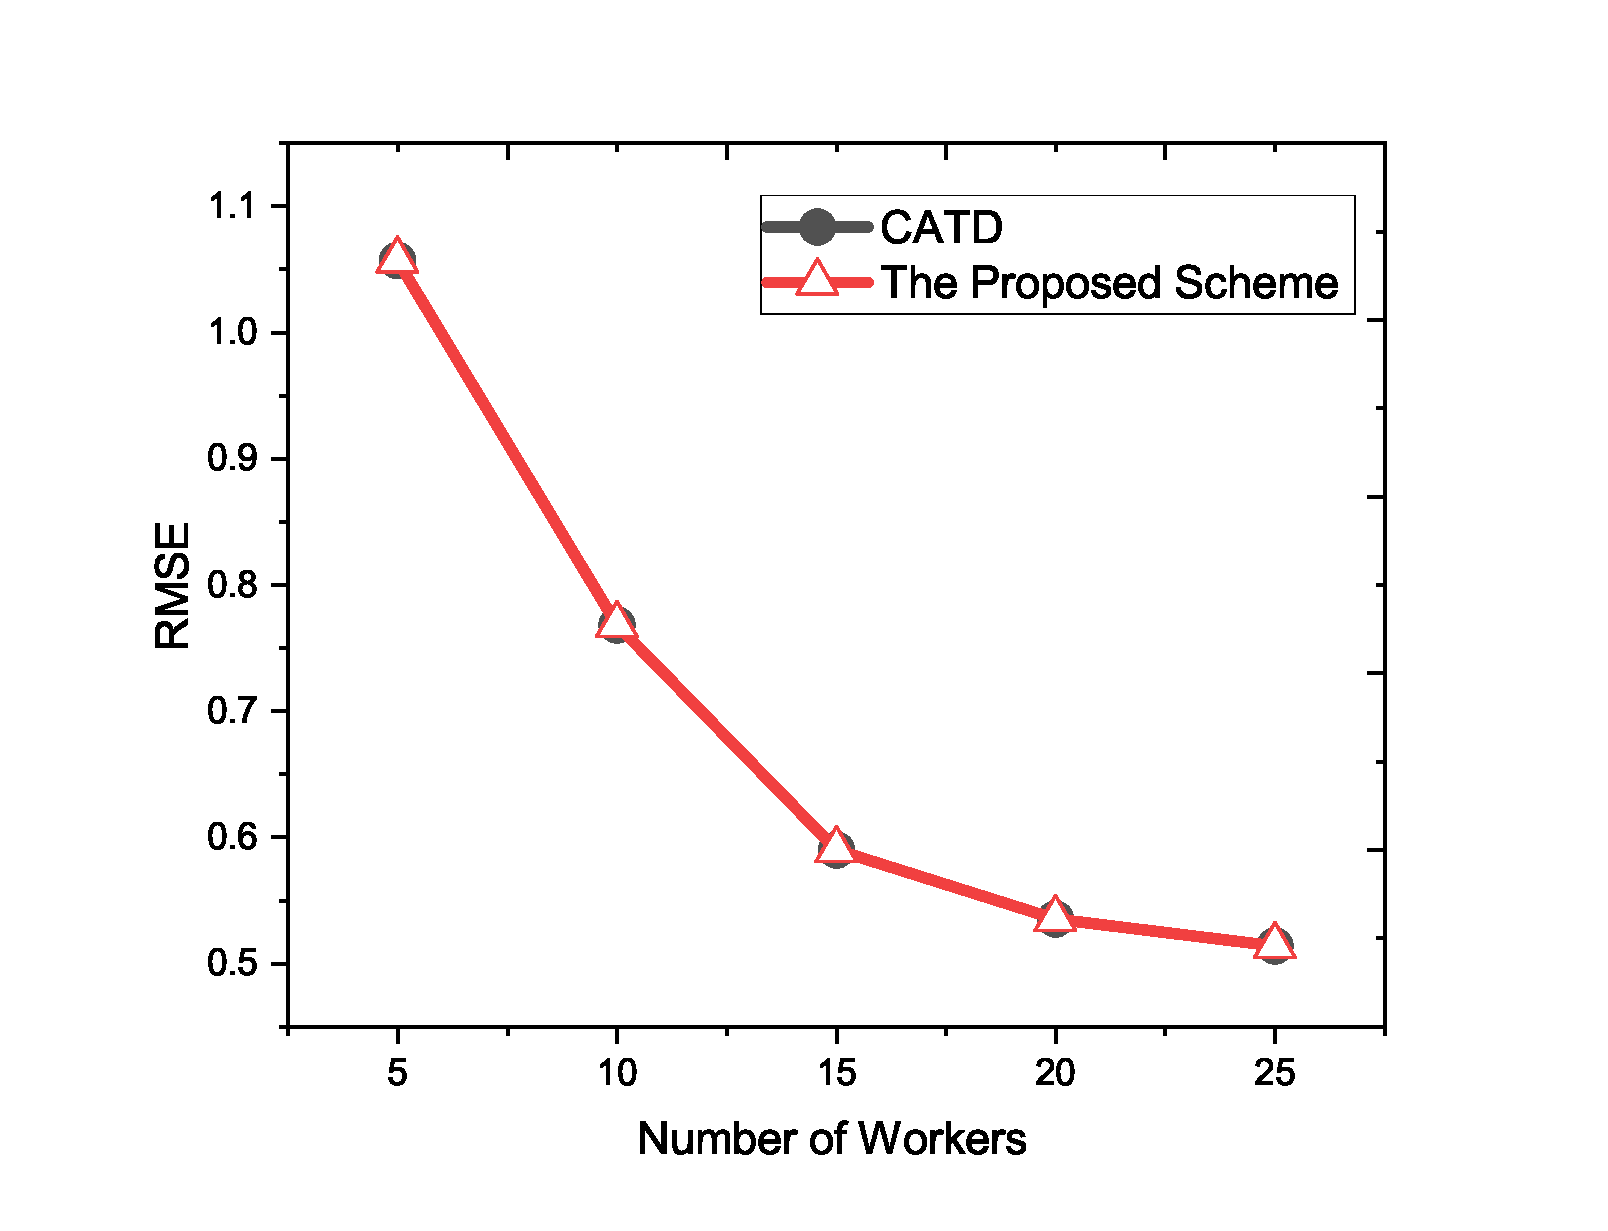
\includegraphics[width=0.5\linewidth]{figures/rmse1.pdf}}
  \subfloat[The Impact of Different Sparsity]{ 
    \label{fig:rmse2} 
    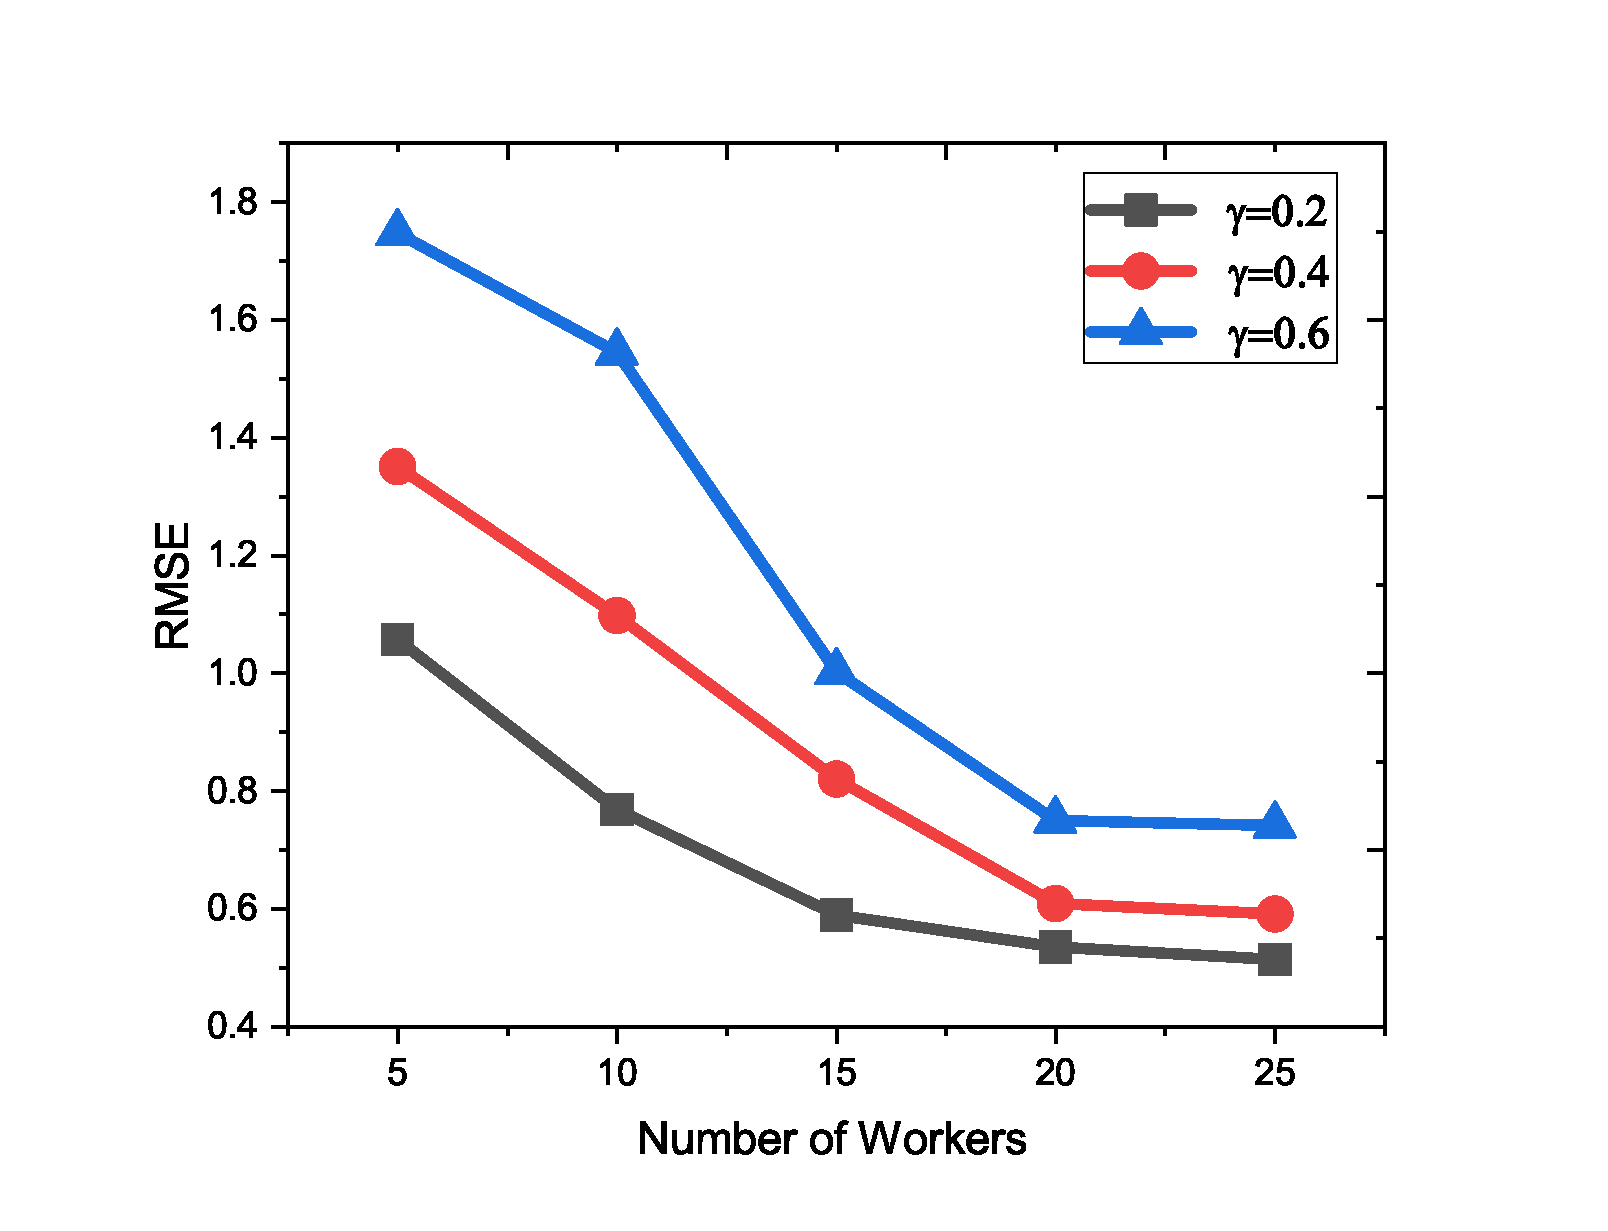
\includegraphics[width=0.5\linewidth]{figures/rmse2.pdf}} 
  \caption{Accuracy Evaluation}
  \label{fig:rmse} 
\end{figure}
To further analyze the impact of sparsity $\gamma$ for accuracy, we conduct the experiment under different sparsity settings from 0.2 to 0.6.
The results in Fig.~\ref{fig:rmse2} show that in a high sparse situation, it is necessary to recruit more workers to decrease the deviation between estimated truths with real ground truths.

\subsection{Convergence}
As for convergence, we use $\sum_{m=1}^M (x_m^t - x_m^{t-1})^2$ as the convergence value in the $t$-th iteration, where $x_m^t$ is the estimated truth in $t$-th iteration and $x_m^0$ is randomly initialized.
In this experiment, the number of workers and objects are fixed as 10 and 20 respectively.
As illustrated in Fig.~\ref{fig:conver}, the convergence speed is very fast at the first few iterations.
Meanwhile, the sparsity has little impact on the convergence.
\begin{figure}[htbp]
  \centering
  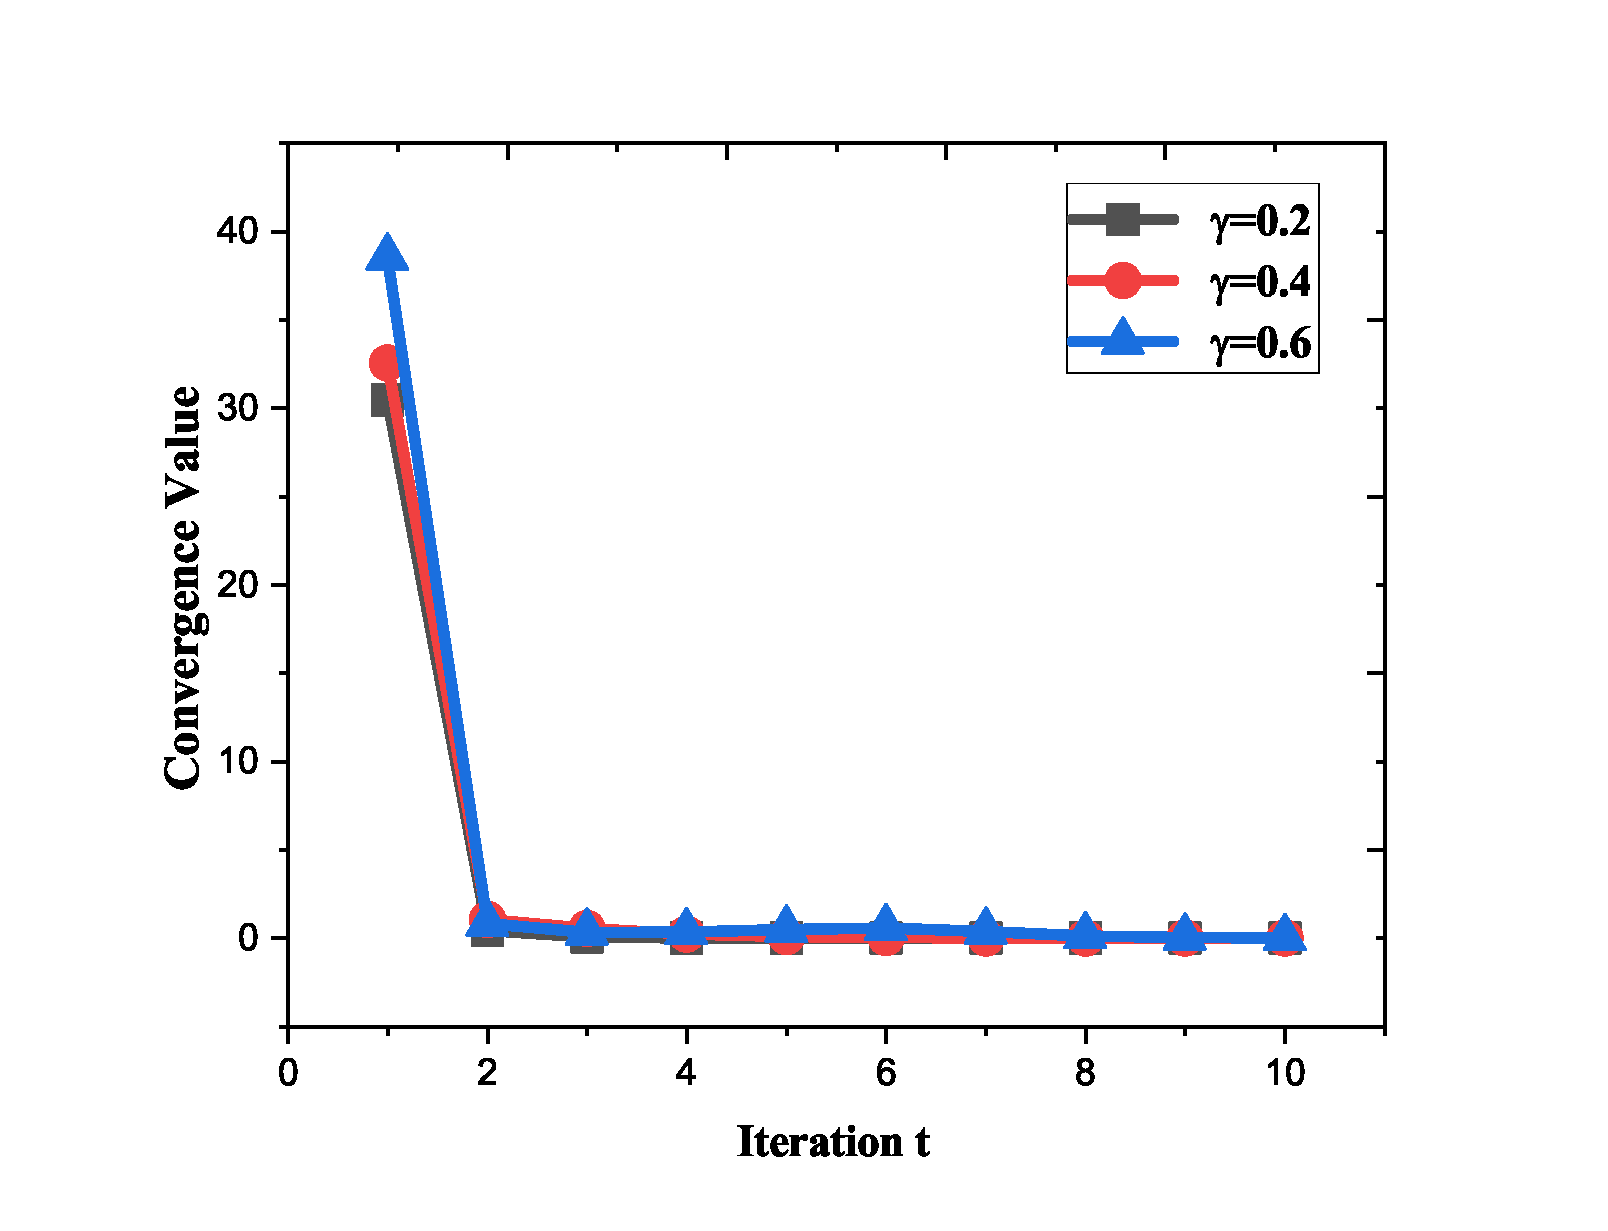
\includegraphics[width=0.75\linewidth]{figures/conver.pdf}
  \caption{Convergence Evaluation}
  \label{fig:conver}
\end{figure}

\subsection{Efficiency Evaluation}
In this part, we measure the performance of computation overhead and communication overhead respectively.
In this experiment, the sparsity is fixed as 0.2 by default.
Hereafter, unless otherwise stated, the default sparsity is set to 0.2.
TABLE~\ref{tab:computation} lists the computation overhead of workers and $S_0$ in non-iteration phases including the report phase and pre-processing phase with the different number of objects and workers.
We observe the computation cost of workers is negligible compared to $S_0$ since there are no heavy cryptographic operations on the workers' side.

\begin{table}[htbp]
  \centering
  \caption{Computation Overhead in Non-Iteration Phases (S)}~\label{tab:computation}
  \linespread{1.3}\selectfont
  \begin{adjustbox}{max width=0.5\textwidth}
  \begin{tabular}{l l c c c}
    \hline
    \hline
    \multicolumn{2}{c}{\multirow{2}*{Number of Workers and Objects}} & \multicolumn{1}{c}{Report Phase} & \multicolumn{1}{c}{Pre-Processing Phase} \\
    \cmidrule(lr){3-3}\cmidrule(lr){4-4} & & Workers & $S_0$ \\
    \hline
     \multirow{3}*{$K=10$} & $M=20$ & 0.0011 & 6.93 \\
      & $M=40$ & 0.0011 & 20.98 \\
      & $M=60$ & 0.0012 & 34.86 \\
     \cmidrule(lr){1-2}
     \multirow{3}*{$M=20$} & $K=20$ & 0.0049 & 14.04\\
     & $K=40$ & 0.0059 & 42.41\\
     & $K=60$ & 0.0104 & 70.92 \\
    \hline
    \hline
  \end{tabular}
  \end{adjustbox}
\end{table}

\begin{figure}[!ht]
  \centering 
  \subfloat[$K = 10 $]{ 
    \label{fig:comp1}
    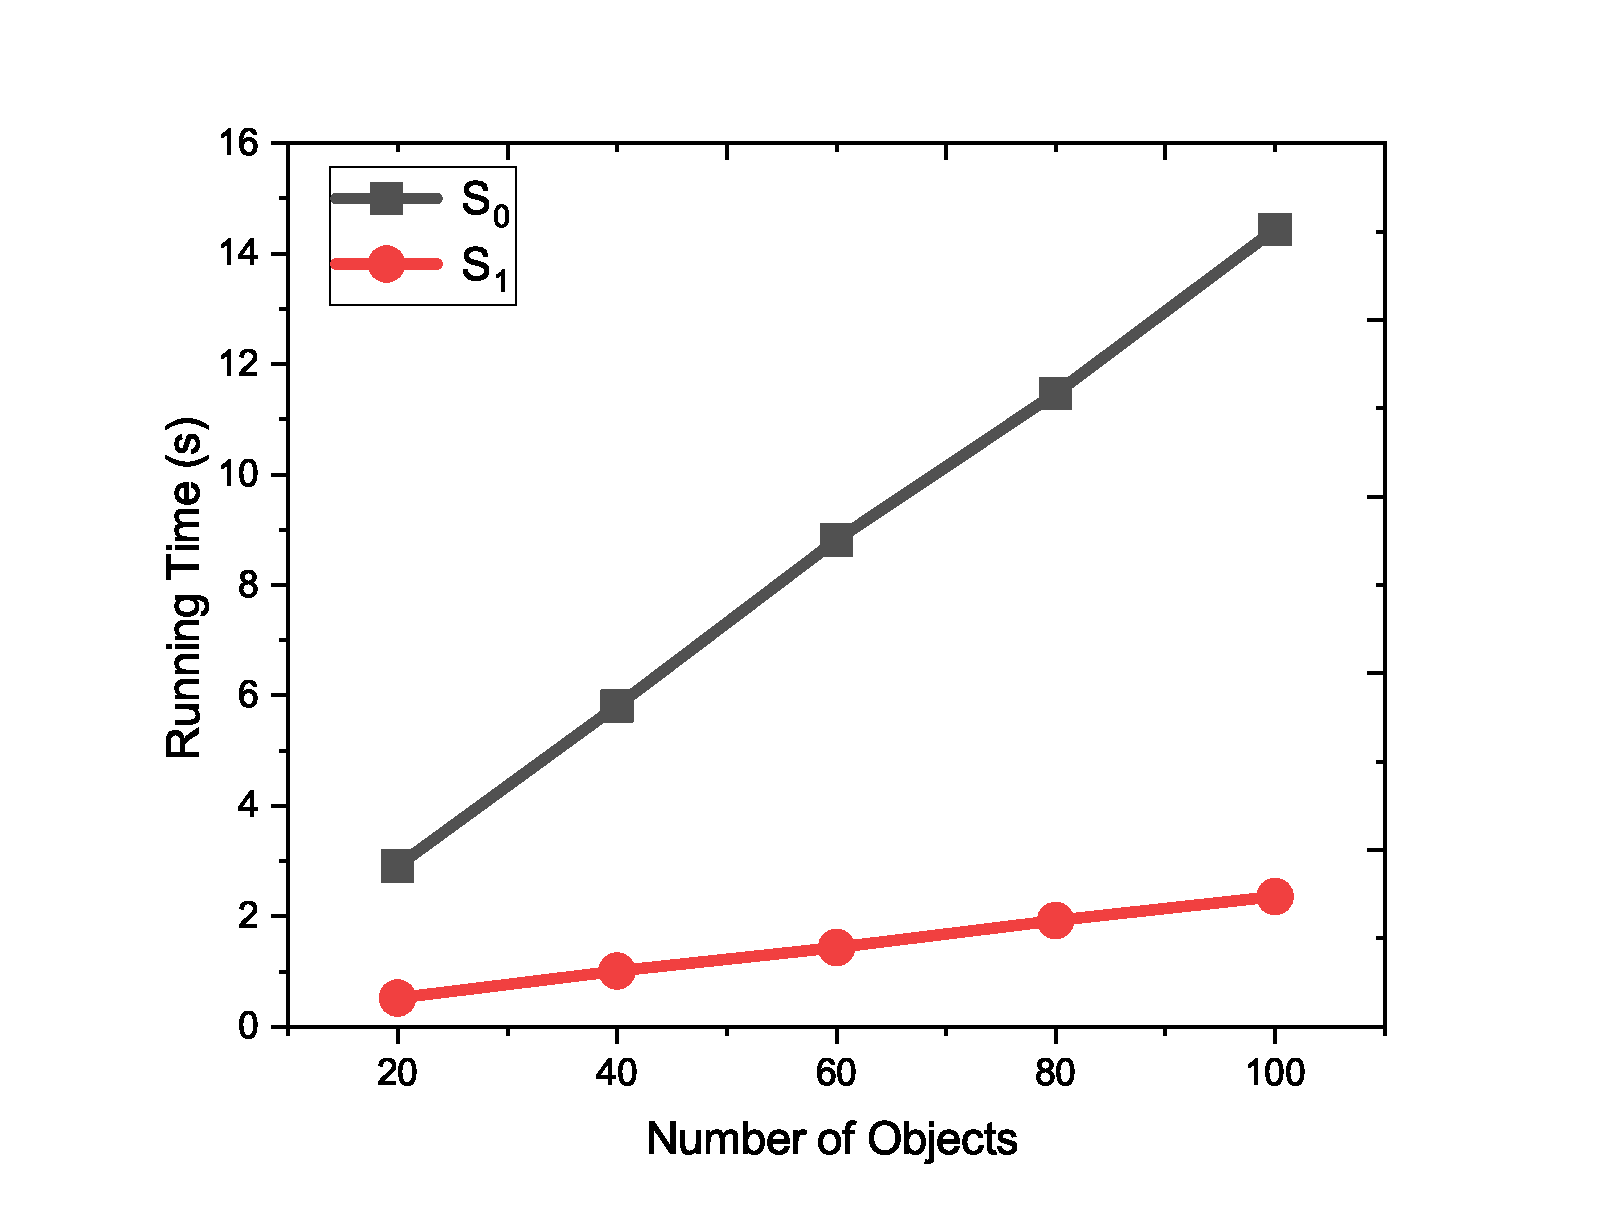
\includegraphics[width=0.5\linewidth]{figures/time_obj.pdf}}
  \subfloat[$M = 20$]{ 
    \label{fig:comp2} 
    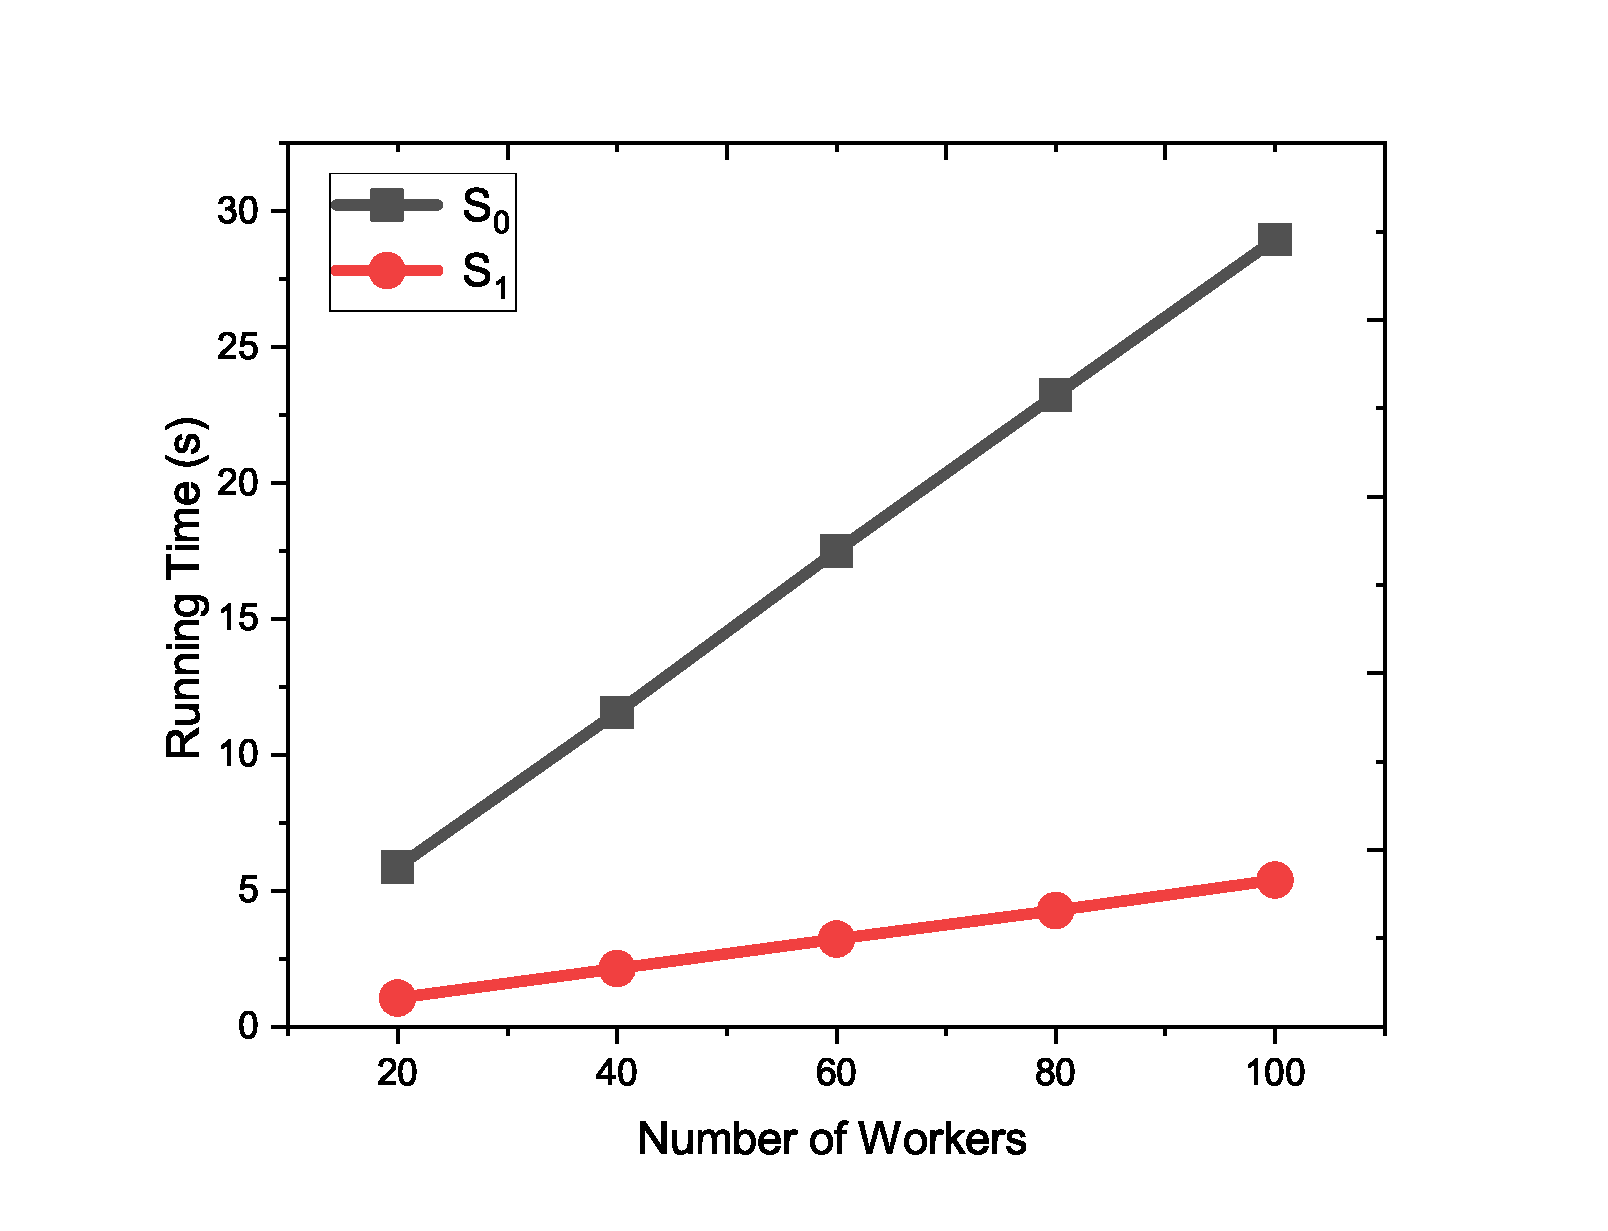
\includegraphics[width=0.5\linewidth]{figures/time_work.pdf}} 
  \caption{Computation Overhead for Each Iteration}
  \label{fig:comp} 
\end{figure}

\begin{table}[!ht]
  \centering
  \caption{Communication Overhead (KB)}~\label{tab:communication}
  \linespread{1.3}\selectfont
  \begin{adjustbox}{max width=0.5\textwidth}
  \begin{tabular}{l l c c c c}
    \hline
    \hline
    \multicolumn{2}{c}{\multirow{2}*{Number of Workers and Objects}} &  \multicolumn{1}{c}{Report Phase} & \multicolumn{1}{c}{Pre-Processing Phase} & \multicolumn{2}{c}{Iteration Phase} \\
    \cmidrule(lr){3-3}\cmidrule(lr){4-4} \cmidrule(lr){5-6} & & Workers to Servers & $S_0$ to $S_1$ & $S_0$ to $S_1$ & $S_1$ to $S_0$ \\
    \hline
    \multirow{3}*{$K=10$} & $M=20$ & 9.60 & 8.08 & 3.44 & 0.04\\
    & $M=40$ & 19.20 & 16.08 & 6.80 & 0.72\\
    & $M=60$ & 28.80 & 24.08 & 10.16 & 1.04\\
    \cmidrule(lr){1-2}
    \multirow{3}*{$M=20$} & $K=20$ & 19.20 & 16.16 & 6.72 & 0.48\\
    & $K=40$ & 38.40 & 32.32 & 13.28 & 0.64 \\
    & $K=60$ & 57.60 & 48.48 & 19.84 & 0.80 \\
    \hline
    \hline
  \end{tabular}
  \end{adjustbox}
\end{table}

As for the iteration phases, we measure the computation cost of $S_0$ and $S_1$ under different numbers of workers and objects for each iteration.
As shown in Fig.~\ref{fig:comp}, the computation cost for $S_1$ is much less compared to $S_0$ in the same conditions.
For the communication overhead, TABLE~\ref{tab:communication} reports the communication overhead for each entity in different phases.
It is clear that the communication overhead in the iteration phase is less than that in the non-iteration phase.
Note that the alternative privacy-preserving truth discovery scheme~\cite{zheng_learning_2018} based on CATD is implemented by GC.
However, the computation cost of GC generation and the communication of GC transmission are huge.
We demonstrate that both computation and communication overheads on the workers' side are lightweight, and the communication overhead between two servers is also acceptable for truth discovery in reality.

\section{Conclusion}\label{sec8}
In this paper, we propose a privacy-preserving truth discovery scheme targeted for privacy-preserving problems in sparse data scenarios.
First, we carefully discuss the privacy issues for truth discovery when sensory data provided by workers are sparse.
After that, we present a scheme to guarantee these requirements by utilizing additively homomorphic cryptosystem based on the CATD framework.
Finally, through the analysis of security, our proposed scheme can provide the strong privacy protection of workers' sensory data, weights, and indicator vectors at the same time.
Extensive experiments also indicate that the computation overhead of workers and the communication overhead in the iteration phase are lightweight enough, which implies that the proposed scheme is practical in real mobile crowdsensing systems.

\bibliographystyle{IEEEtran}
\bibliography{ref}

\vspace{12pt}

\end{document}